\documentclass[]{article}

\title{Canyon: Permanent Storage Layer for Web3}
\author{
    Liu-Cheng Xu\\
    \\
    \textit{Canyon Labs}
}
\date{}

\usepackage{amsmath}
\usepackage{hyperref}
\usepackage[firstpage]{draftwatermark}
\SetWatermarkLightness{0.4}
\SetWatermarkFontSize{6cm}
\SetWatermarkText{Draft}

\usepackage{tikz}

%\usepackage{algorithm}
%\usepackage{algorithmic}
\usepackage[linesnumbered,boxed,ruled,commentsnumbered]{algorithm2e}

\usepackage{xcolor}

% Use for advanced enum-list functionality
\usepackage{enumitem}

% Define question and answer environment
\newenvironment{faq}{\begin{description}[style=nextline]}{\end{description}}

\usepackage[a4paper,left=3cm,right=3cm,top=3cm,bottom=3cm]{geometry}
\usepackage{algpseudocode}

\setlength{\parskip}{0.6em}

\usepackage{titlesec}
\titleclass{\subsubsubsection}{straight}[\subsection]

\usepackage{xcolor}
\usepackage{soul}

\definecolor{inlineBG}{HTML}{F1F1F1}
\definecolor{inlineFG}{HTML}{FF0000}
\newcommand{\code}[1]{{%
  \sethlcolor{inlineBG}%
  \color{inlineFG}%
  \ttfamily
  \hl{ #1 }%
}}

\newcounter{subsubsubsection}[subsubsection]
\renewcommand\thesubsubsubsection{\thesubsubsection.\arabic{subsubsubsection}}
\renewcommand\theparagraph{\thesubsubsubsection.\arabic{paragraph}}

\titleformat{\subsubsubsection}
  {\normalfont\normalsize\bfseries}{\thesubsubsubsection}{1em}{}
\titlespacing*{\subsubsubsection}
{0pt}{3.25ex plus 1ex minus .2ex}{1.5ex plus .2ex}

\makeatletter
\renewcommand\paragraph{\@startsection{paragraph}{5}{\z@}%
  {3.25ex \@plus1ex \@minus.2ex}%
  {-1em}%
  {\normalfont\normalsize\bfseries}}
\renewcommand\subparagraph{\@startsection{subparagraph}{6}{\parindent}%
  {3.25ex \@plus1ex \@minus .2ex}%
  {-1em}%
  {\normalfont\normalsize\bfseries}}
\def\toclevel@subsubsubsection{4}
\def\toclevel@paragraph{5}
\def\toclevel@paragraph{6}
\def\l@subsubsubsection{\@dottedtocline{4}{7em}{4em}}
\def\l@paragraph{\@dottedtocline{5}{10em}{5em}}
\def\l@subparagraph{\@dottedtocline{6}{14em}{6em}}
\makeatother

\setcounter{secnumdepth}{4}

% \usepackage[active,tightpage]{preview}
% \PreviewEnvironment{tikzpicture}
% \setlength{\PreviewBorder}{10pt}%

\usetikzlibrary{arrows}

\tikzset{
  basenode/.style = {align=center, inner sep=4pt, text centered},
  root_node/.style = {basenode, rectangle, draw=black, text width=6em},
  tree_node/.style = {basenode, rectangle, draw=black, text width=4em},
  c_node/.style = {basenode, rectangle, dashed, draw=black, text width=4em, very thick},
  leaf_node/.style = {basenode, rectangle, draw=black, text width=2em},
  chunk_leaf_node/.style = {basenode, rectangle, fill=gray, draw=black, text width=2em},
  t_node/.style = {basenode, rectangle, red, fill=green, draw=black, text width=2em},
  proof_node/.style = {basenode, rectangle, draw=blue, text width=2em, very thick},
}

\begin{document}

\maketitle

\begin{abstract}

Canyon is a permanent storage network built on Substrate, which records the hashes of files on-chain and stores the files off-chain. By blending PoS and a probabilistic proof-of-storage scheme inspired by Arweave, Canyon greatly reduces the barriers to entry for miners, who are incentivized to store as much data as possible for the rewards.

\end{abstract}

\tableofcontents

\newpage

\section{Introduction}

\subsection{Motivation}

It can't be denied that the storage infrastrusture will be an essential part of Web3 in the future.

% \subsection{Organization}

% TODO

\section{Background}

\subsection{Filecoin}

Filecoin\cite{ref1} proposes a sophisticated cryptographic solution based on zero-knowledge proofs (ZKPs) to prevent the common attacks on the decentralized storage verification, which uses pure mathematical methods and is able to achieve high-security guarantees. The whole mining process consumes too much computing power, rendering the actual storage cost prohibitively expensive. Furthermore, the high hardware requirements largely raise the threshold for small miners, preventing those with pure common commodity hardware from joining the network, the storage distribution today becomes centralized.

Due to the lack of authentic storage needs and system design of Filecoin, the miners themselves are economically impelled to store tons of garbage data in the network, increasing the storage power and maximizing their mining profit. Despite the Filecoin team has proposed the off-chain governance approach like Filecoin Plus\footnote{\url{https://docs.filecoin.io/store/filecoin-plus}}, it does not mitigate this problem substantially, leaving the promotion of the useful storage still a huge unresolved challenge in the Filecoin network.

\subsection{Crust}

To solve the problem of decentralized storage verification, Crust\cite{ref2} adopts a hardware-based solution Trusted Environment Execution (TEE) to make sure the miners store a specific number of data copies as promised. Each of the storage nodes is required to enroll on Crust chain through TEE before it's allowed to deal with the storage orders from client. The TEE module of the nodes will periodically check and report whether the files are properly stored in the local storage space in a trusted way.

There are three major TEE providers with different implementations: Software Guard Extensions (SGX) on the Intel platform, Secure Encrypted Virtualization (SEV) on the AMD platform, and TrustZone on the ARM platform. The SGX of Intel is the most widely used TEE platform. Although Crust has a relatively low hardware demand for mining compared with Filecoin, the miners are heavily dependent on a fairly narrow range of hardware that supports TEE, thus being greatly affected by the hardware manufacturers.

\subsection{Arweave}

Unlike the ephemeral storage services such as Filecoin, Crust, Arweave\cite{ref3} serves as a permanent storage layer using a probabilistic and incentive-driven approach to maximize the number of redundant copies of any individual piece of data in the network, which fills in a crucial aspect of decentralized storage need in Web 3.0. The natural feature of perpetual storage is perfectly suitable for the NFTs, and is the cornerstone of new storage-based computation paradigm like everFinance \footnote{\url{https://medium.com/everfinance/a-storage-based-computation-paradigm-enabled-by-arweave-de799ae8c424}}.

Without the periodical audit of the data replicas, Arweave is much effortless than the other solutions in terms of the constraint and cost of storage consensus. Nevertheless, the deficiency of this scheme is the potential risk of data centralization that ultimately there possibly will be a single storage provider serves the whole data. The Arweave team has introduced and deplopyed an improved version of consensus Succinct Proofs of Random Access, attempting to disincentivize miners from retrieving data on demand from the network.

\section{Design Principles\\
}

\subsection{Security and Privacy}

\section{System Design}

\subsection{Consensus}

Canyon network is profoundly inspired by Arweave, especially the storage consensus, aiming to be a permanant decentralized storage network using the Substrate framework. The key contribution of Canyon is that it adapts PoS into the storage consensus of Arweave, whereas Arweave uses PoW, making Canyon a more scalable and environment-friendly network.

In order to mine a block, a legitimate POA, which proves the block author has the access to the data of a random historical block, is required to be included in the block header. According to the computed result of POA, we can estimate the proportion of data stored locally by a node in the network-wide data. Based on this, we link the PoS rewards to the estimated storage capacity of a node. The more data a node stores, the more rewards it can receive. Besides, as the number of blocks mined by the node continues to grow, the estimation of the node's storage capacity will be getting closer to the actual value.

\subsubsection{Proof of Access}

In Arweave, the probability that a node can mine a block is a function of the node’s hashing power relative to the average hashing power of all of the nodes in the network that also possess the recall block.

\begin{flalign}
  \hspace{5mm}   P(\text{win}) = P(\text{has recall block}) * P(\text{finds hash first})
\end{flalign}

In Canyon, a PoS-based system, the node is allowed to produce a block only when it succeeds in claiming the slot and owns the data of recall block:

\begin{flalign}
    \hspace{5mm}   P(\text{win}) = P(\text{has recall block}) * P(\text{claims slot})
\end{flalign}

\IncMargin{1em}
\begin{algorithm}
    \label{algo:poa}

    \SetAlgoNoLine
    \SetKwInOut{Input}{\textbf{Input}}\SetKwInOut{Output}{\textbf{Output}}

    \Input{
        \\
        The random seed $S$\;\\
        The weave size $W$\;\\}
    \Output{
        \\
        The proof of accessing the recall block $POA$\;\\}
    \BlankLine

    Initialize the number of repeats $x$ with 1\;
    \BlankLine

    \Repeat
        {\text{The data of TX is available}}
        {
        Draw a random byte $B$ with $\Call{MultiHash}{S, x} \mod W$\;
        Find the $TX$ in which the random byte $B$ is included\;
        {$x \leftarrow x + 1$}\;
    }

    \BlankLine
    $POA \leftarrow \Call{ConstructPOA}{TX}$\;
    \Return $POA$\;
    \caption{Generation of POA}
\end{algorithm}
\DecMargin{1em}

The steps for generating the storage proof are as follows\footnote{This version is currently based on the initial consensus of Arweave Proof of Access instead of the new one Succinct Proofs of Random Access. The most noticeable change in SPoRA upgrade is that the miners now have to compute a slow hash to locate the random recall byte, rendering those who request data from the remote storage pool at a distinct disadvantage. To put it simply, $\Call{MultiHash}{S, x}$ in \ref{algo:poa}{ Algo 1} is replaced with a new slow hash.}:

\begin{enumerate}
    \item Input the value of \code{parent\_hash} and \code{weave\_size} respectively. And \code{depth} is initialized to 1.
  \item Compute \code{recall\_byte}, i.e. a random byte in the network-wide data history ranging from 0 to \code{weave\_size}, excluding \code{weave\_size}.
  \item Find out the \code{recall\_tx} the contains the \code{recall\_byte} computed from the previous step.
  \item If the miner already has stored the data of \code{recall\_tx} locally, extract the original data of \code{recall\_tx} and split the data into a list of chunks, then construct a storage proof \code{poa \{ depth, tx\_path, chunk\_root, chunk\_path, chunk \} }(See \ref{poa}{ poa Data Structure }).
  \item If the miner does not have the data of \code{recall\_tx} locally, increase the value of \code{depth} by 1 and repeat the step 2 to 4.
  \item Return \textbf{poa}.
\end{enumerate}

As you can see, if a node stores 100\% of data, the value of \code{depth} always remains 1. The node only needs to go through the above steps once every time when it attempts to generate a \code{poa} proof. If the node stores 50\% of data, the value of \code{depth} is expected to approach 2 as it produces enough blocks. If the node stores 10\% of data, the value of \code{depth} approaches 10.

If a node produces a total of $N$ blocks, and the poa.depth of each block is $depth_{i\in 1,2,...,N}$, the average \code{depth} value of the $N$ blocks $\hat{x}$ is:

$$
\hat{x} = \frac{1}{N} {\sum_{i=1}^N x_i}
$$

With time, the node produces enough blocks (i.e. $N \to \infty$), we can calculate the proportion of data stored locally by the node relative to the network-wide data more precisely with the value of $\hat{x}_{N \to \infty}$. The formula is as follows:

$$
R = \frac{1}{\hat{x}_{{N \to \infty}}}
$$

With the knowledge of the storage capacity of nodes $R$, we can incentivize the miners to store more users' data by allocating the rewards accordingly.

\subsubsection{Proof of Stake}

\subsubsubsection{Validator Election}

The validators on Canyon network have two responsibilities: author blocks as a virtual miner and provide unstoppable storage services. The security of a PoS system is rooted in the number of tokens locked in the staking pool.

\subsubsubsection{Staking Rewards}

The reward for a miner producing a block is composed of three parts:

$$
R_{total} = R_{inflation} + R_{fees} + R_{endowment}
$$

\subsection{Economy Model}

\subsubsection{Bandwidth}

For any storage platform to be valuable, it must be careful not to lose the data it was given, even in the presence of a variety of possible failures within the system. What's more, a storage platform is of no use unless it also functions as a retrieval platform. Only when the data can be retrieved without any pains whenever the client wants to can we hope a fully functional storage service.

\subsubsection{Transaction Fee}

The fee of data storage transaction is composed of the perpetual storage cost and one-shot bandwidth cost. The perpetual storage cost is basically modeled after Arweave, on the observed pattern that the cost of commercially available storage media has been decreasing at a significant rate over the last decades and this trend is foreseed to last for hundreds of years.

\subsubsection{Data Oblivion}

Specifically, the perpetual storage needs can be classified into two kinds: immortal and indefinite storage. The immortal storage means the file that is doomed to be preserved from the creation, such as the metadata of NFTs. Indefinite storage is such a kind of data that has an uncertainty of ending time, but can be deleted once it's used or the client simply does not wish the contract to be continued for any reason.

For these use cases, Canyon allows the origin uploader opts to terminate the contract and partially refund the charged perpetual storage fee. The files that have been refunded will be disqualified to be selected for the future storage consensus procedure, thus the miners that keep storing them will receive no rewards. For the sake of scarce storage resources, the miners are expected to purge these data from local storage, consequently, sooner or later, the data will be eliminated from the network.

\subsubsection{Payments}

An inherent advantage of Canyon is the easier interoperability with the Polkadot\cite{ref4} ecosystem by using Substrate\cite{ref5}, which is the same framework Polkadot is built on. Apart from the native token of Canyon CYN, Canyon will support the users pay the storage fee by introducing the stable coins like USDT from Polkadot network, reducing the impact of the churn of token price on providing a stable storage service for the custom.

\section{Conclusion}

Canyon network is designed to be a permanent decentralized storage network, putting the emphasis on both light-weight storage consensus and highly-avaliable data retrieval. Being a permanent storage layer, Canyon is better suited for the storage-based computation paradigm.

\begin{thebibliography}{99}
\bibitem{ref1}Protocol Labs, Filecoin: A Decentralized Storage Network, \url{https://filecoin.io/filecoin.pdf}.
\bibitem{ref2}\url{https://crust.network/}
\bibitem{ref3}Sam Williams, Viktor Diordiiev, Lev Berman, India Raybould, Ivan Uemlianin. Arweave: A Protocol for Economically Sustainable Information Permanence.
\bibitem{ref4}Gavid wood. Polkadot: Vision for A Heterogeneous Multi-chain Framework. \url{https://polkadot.network/PolkaDotPaper.pdf}
\bibitem{ref5}Substrate: The platform for blockchain innovators. \url{https://github.com/paritytech/substrate}
\end{thebibliography}

\appendix
\section{Appendix}

\subsection{Data Structure}

\subsubsection{poa}\label{poa}

Each storage proof is composed of the following fields:

\begin{itemize}
    \item \textit{depth}: the number of total attempts to construct a valid poa for producing block.
    \item \textit{tx\_path}: Merkle path of recall transaction to the transaction root, which is included in the block header.
    \item \textit{chunk\_root}: Merkle root of transaction data chunks.
    \item \textit{chunk\_path}: Merkle path of \textit{chunk} to \textit{chunk\_root}.
    \item \textit{chunk}: Raw bytes of recall chunk, at most 256 KiB.
\end{itemize}

Technically, the way to prove the miner did store the data of recall block, is that it can be verifiably proved that the miner holds one piece of data belonging to that block, which requires two merkle proofs to be generated: \textit{tx\_path} and \textit{chunk\_path}. With the origin \textit{chunk}, anyone can verify that the block author did have access to the data of recall transaction without downloading the entire data of that block. Furthermore, everyone can verify the storage proof by merely downloading the block header, for the full content of poa is included in the header as a digest item.

\begin{figure}
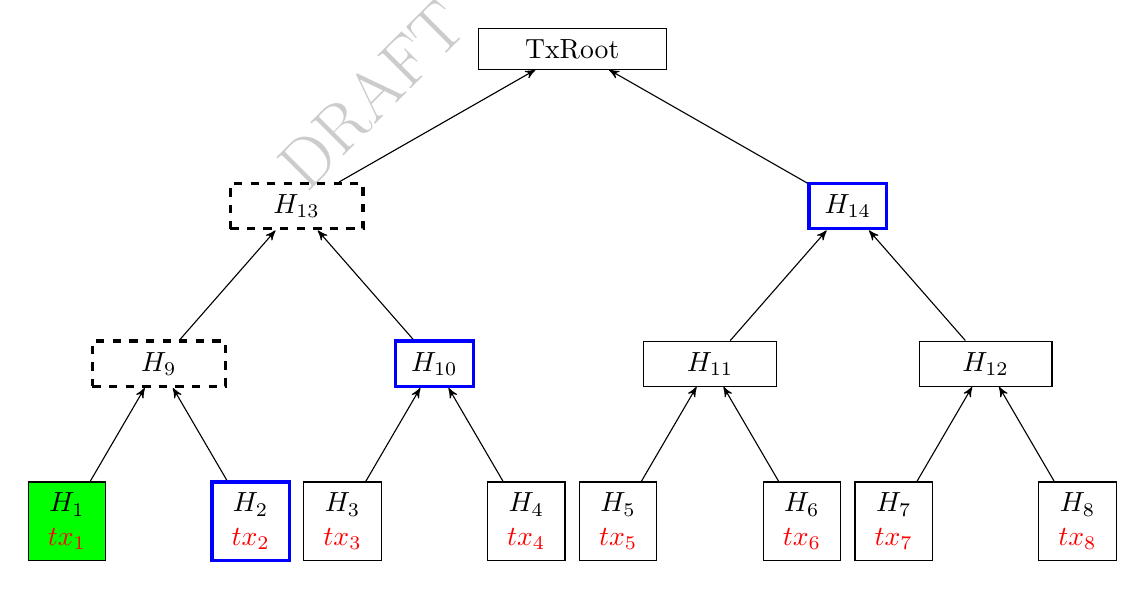
\begin{tikzpicture}[<-,>=stealth',level/.style={sibling distance = 7cm/#1, level distance = 2cm}]
    \node [root_node] {TxRoot}
    child{ node [c_node] {$H_{13}$}
            child{ node [c_node] {$H_{9}$}
                child{ node [t_node] {{\color{black}{$H_1$}} $tx_1$}}
                child{ node [proof_node] {$H_2$ \color{red}{$tx_2$}}}
            }
            child{ node [proof_node] {$H_{10}$}
                child{ node [leaf_node] {{\color{black}{$H_3$}} \color{red}{$tx_3$}}}
                child{ node [leaf_node] {{\color{black}{$H_4$}} \color{red}{$tx_4$}}}
            }
    }
    child{ node [proof_node] {$H_{14}$}
            child{ node [tree_node] {$H_{11}$}
                child{ node [leaf_node] {{\color{black}{$H_5$}} \color{red}{$tx_5$}}}
                child{ node [leaf_node] {{\color{black}{$H_6$}} \color{red}{$tx_6$}}}
            }
            child{ node [tree_node] {$H_{12}$}
                child{ node [leaf_node] {{\color{black}{$H_7$}} \color{red}{$tx_7$}}}
                child{ node [leaf_node] {{\color{black}{$H_8$}} \color{red}{$tx_8$}}}
            }
    }
;
\end{tikzpicture}
\caption{Tx Path}
\end{figure}

Assuming the recall byte is located in the chunk $C_4$ which is part of the data of $tx1$.

\begin{figure}
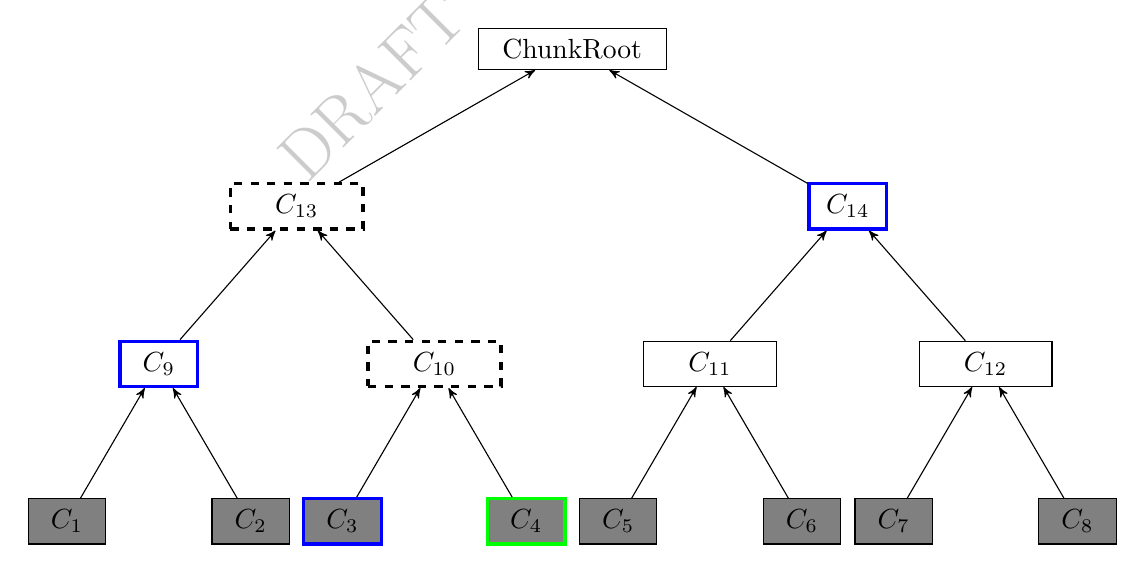
\begin{tikzpicture}[<-,>=stealth',level/.style={sibling distance = 7cm/#1, level distance = 2cm}]
    \node [root_node] {ChunkRoot}
    child{ node [c_node] {$C_{13}$}
            child{ node [proof_node] {$C_{9}$}
                child{ node [chunk_leaf_node] {$C_1$}}
                child{ node [chunk_leaf_node] {$C_2$}}
            }
            child{ node [c_node] {$C_{10}$}
                child{ node [align=center, inner sep=4pt, text centered, rectangle, fill=gray, draw=blue, text width=2em, very thick] {$C_3$}}
                child{ node [align=center, inner sep=4pt, text centered, rectangle, fill=gray, draw=green, text width=2em, very thick] {$C_4$}}
            }
    }
    child{ node [proof_node] {$C_{14}$}
            child{ node [tree_node] {$C_{11}$}
                child{ node [chunk_leaf_node] {$C_5$}}
                child{ node [chunk_leaf_node] {$C_6$}}
            }
            child{ node [tree_node] {$C_{12}$}
                child{ node [chunk_leaf_node] {$C_7$}}
                child{ node [chunk_leaf_node] {$C_8$}}
            }
    }
;
\end{tikzpicture}
    \caption{Chunk Path: the transaction data of $tx_1$ is segmented into 256-kilobyte chunks(gray).}
\end{figure}

\end{document}
